\documentclass[12pt]{article}
\usepackage{amsmath,mlmodern}
\usepackage{graphicx, float} % Required for inserting images
\usepackage[english]{babel}
\usepackage{amsthm}
\usepackage{amssymb}
% \usepackage{fullpage}
\usepackage[a4paper, right = 0.8in, left = 0.8in, top=0.5in, bottom = 0.2in]{geometry}
\usepackage[protrusion=true,expansion=true]{microtype}	
\usepackage{pgfplots}

\usepackage{subfiles}

\pgfplotsset{width=10cm,compat=1.9}
\usepgfplotslibrary{external}
\tikzexternalize

\newtheorem{theorem}{Theorem}[section]
\newtheorem{corollary}{Corollary}[theorem]
\newtheorem{lemma}[theorem]{Lemma}

\theoremstyle{definition}
\newtheorem{definition}{Definition}[section]

\theoremstyle{definition}
\newtheorem{example}{Example}[section]

\theoremstyle{remark}
\newtheorem*{remark}{Remark}

% \renewcommand\qedsymbol{$\blacksquare$} // For QED symbol

\begin{document}
\title{LS2102: Biology Laboratory \\[2ex] LAB REPORT 2}
\author{Sabarno Saha \\Roll No. 22MS037}
\date{\today}

\maketitle
\tableofcontents
\newpage
\section{Aim}
To determine the unknown concentration of p-NPP(para-Nitrophenylphosphate) and determine the enzymatic properties of Alkaline Phosphatase enzyme.
\section{Procedure}
\subsection{Preparation of Standard Curve}
\begin{enumerate}
    \item Solutions of different concentrations (containing buffer, pNP and NaOH), having
different amount of pNP were prepared.
\item  Absorbance of each solution was taken at 405nm.
\item Graph of Absorbance vs. Concentration of pNP was plotted and fit with a $Ax+B$.
\item The value of slope and intercept from the fit curve was noted.
\end{enumerate}

\subsection{Estimation of Kinetic Parameters}
\begin{enumerate}
    \item The buffer, enzyme and substrate solutions were prepared according to the table
provided.
\item  The solutions were kept for incubation at 300K for 15 minutes.
\item  Absorbance at 405nm was taken for each solution.
\item The reaction velocities were calculated by obtaining product at the specified absorbance from the standard linear fitting $Ax+b$ done in the previous step.
\item The Michaelis-Menton Curve was plotted with fit $\dfrac{Ax}{B+x}$
\item The Lineweaver-Burke Curve were plotted with again a standard linear fit
\item From the curve, various kinetic parameters were calculated.
\end{enumerate} 

\section{Data Tables and Graphs}
\subsection{Data Table to Prepare Standard Absorbance vs pNP Curve}
\begin{center}
    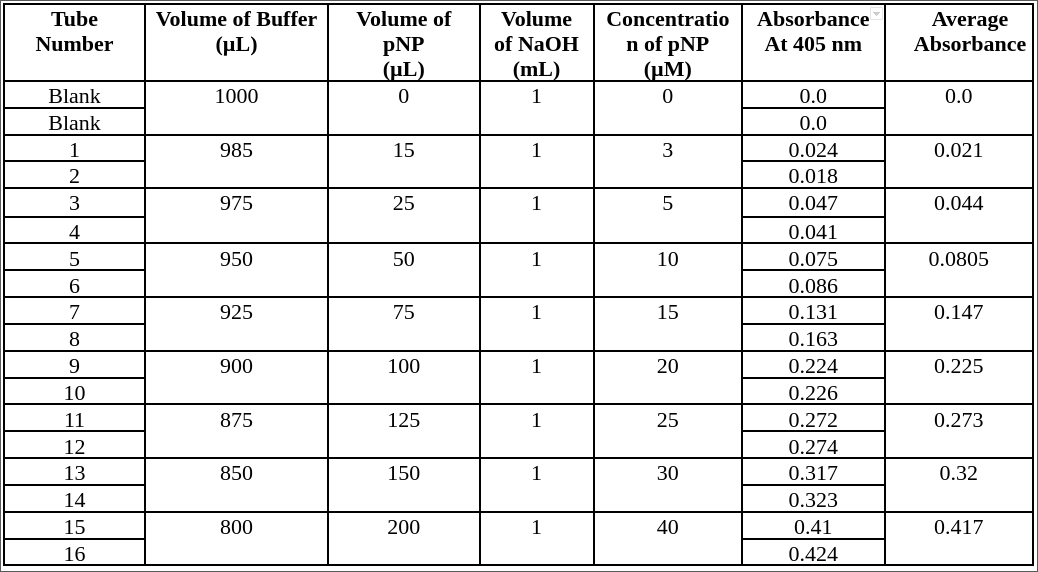
\includegraphics[width = 6.0in]{Pasted image 1.png}
\end{center}
% Please add the following required packages to your document preamble:
% \usepackage{multirow}
% Please add the following required packages to your document preamble:
% \usepackage{multirow}

\subsection{Table 2(Kinetic Parameters)}
\begin{center}
    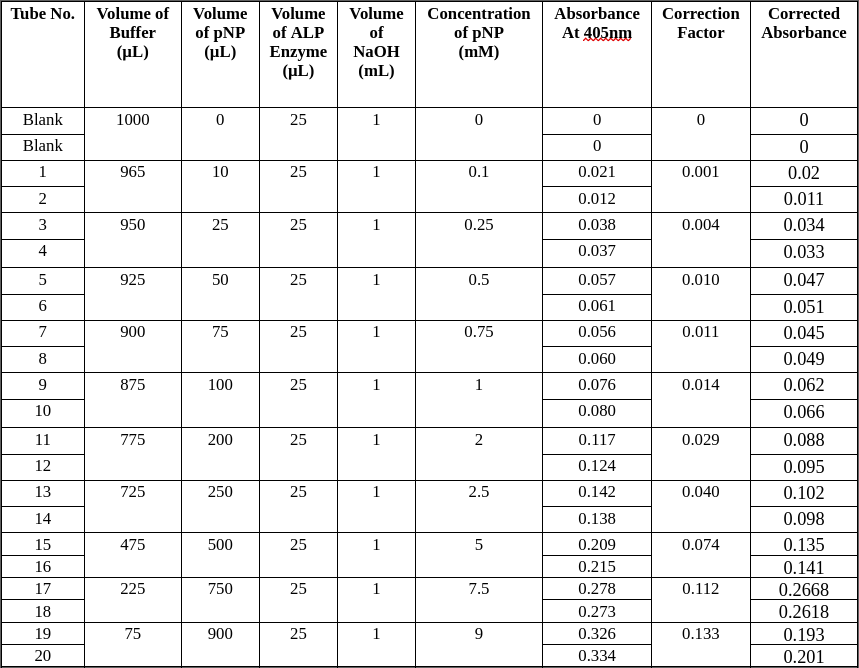
\includegraphics[width = 6.0in]{Pasted image 2.png}
\end{center}
\subsection{Table 3(Kinetic Parameters)}
\begin{center}
    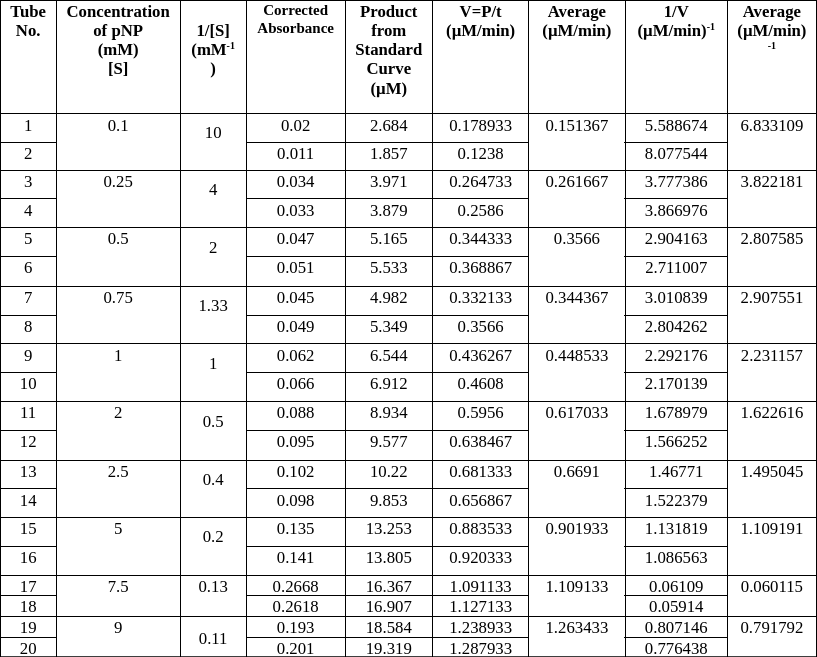
\includegraphics[width = 6.0in]{Pasted image 3.png}
\end{center}

\subsection{Graphs}
\begin{figure}[H]
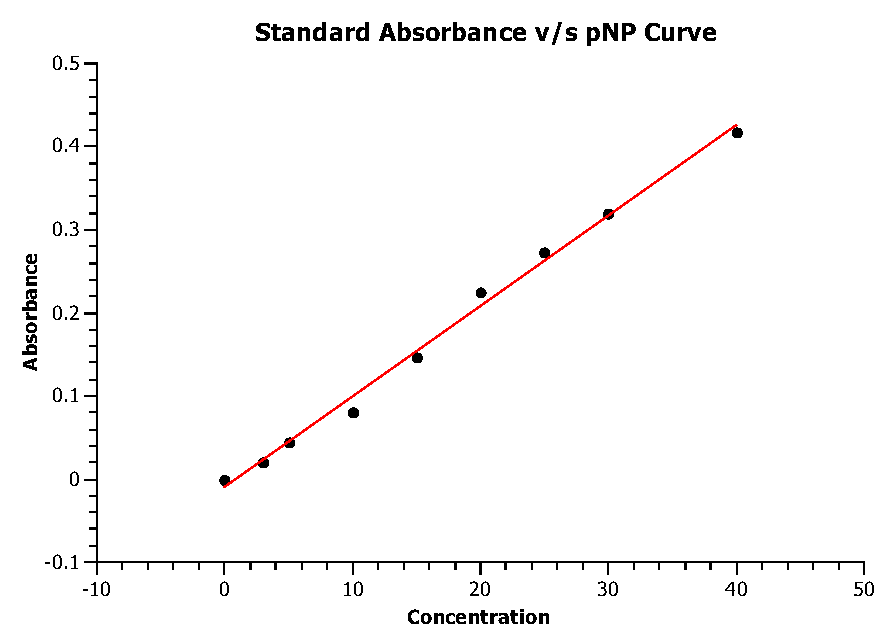
\includegraphics[width=16cm]{Graphstandard.eps}
\centering
From fitting the line of the curve as per the equation Ax+B we get the values of A,B as:-\\[2ex]
B (y-intercept) = -9.2011952191235e-03 \\
A (slope) = 1.0880478087649e-02 
\end{figure}
\begin{figure}[H]
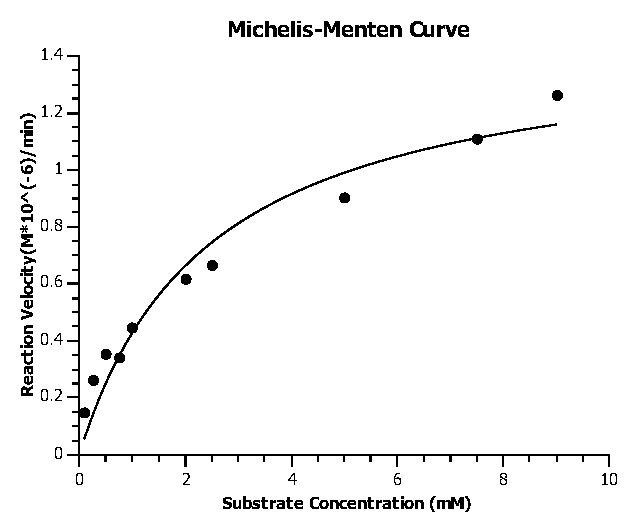
\includegraphics[width=16cm]{Graphst2.eps}
\centering
From fitting the line of the curve as per the equation $\dfrac{Ax}{B+x}$ we get the values of A,B as:-\\[2ex] 
B = 2.45 \\ 
A = 1.47 
\end{figure}
\begin{figure}[H]
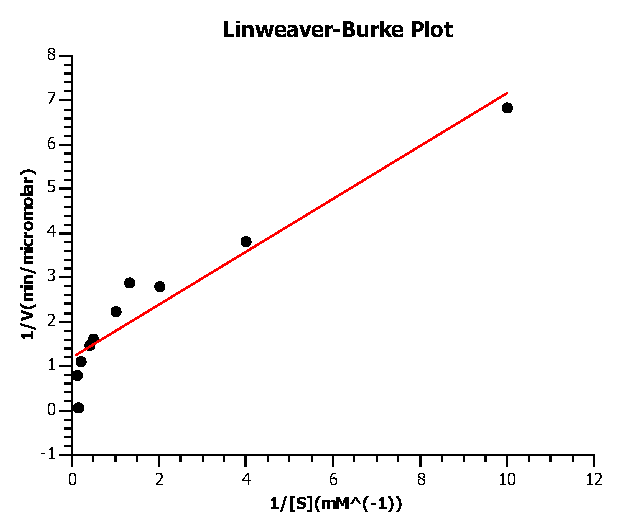
\includegraphics[width=16cm]{Graph23.eps}
\centering
From fitting the line of the curve as per the equation Ax+B we get the values of A,B as:-\\[2ex]
B (y-intercept) = 1.19\\
A (slope) = 0.597
\end{figure}
\section{Calculations and Results}

From the graph we found out that \\

$V_{max}=\dfrac{1}{B}=0.840 \mu $M/min. \\

$K_{max}=A*V_{max}=0.502$ mM\\


$[E]_{T}= \dfrac{\text{Volume of Enzyme taken}}{\text{Total Volume}} \times \text{Concentration of Stock} = 0.504  \mu$M \\

$k_{cat}=1.67 $  min$^{-1}$\\

Specific Activity of the enzyme = $\dfrac{0.840*1}{0.00025} = 3,360
  \mu ~mol~ min^{-1}~mg^{-1}$


\newpage
\section{Results}
Thus with the help of Michelis-Menten Curve and Linweaver-Burke Plot we could figure out the various kinetic parameters of the enzyme alkaline phosphate and the results are given below
\begin{center}
$V_{max}=0.840 \mu $M/min. \\

$K_{max}=0.502$ mM\\


$[E]_{T}= 0.504  \mu$M \\

$k_{cat}=1.67 $  min$^{-1}$\\

Specific Activity of the enzyme =  3,360 $\mu ~mol~ min^{-1}~mg^{-1}$
\end{center}
\end{document}

